% ==========================================
% BAB V IMPLEMENTASI
% ==========================================
\cleardoublepage
\chapter{IMPLEMENTASI}
\label{chap:implementasi}

\section{Lingkungan Implementasi}
Sistem pencarian foto pribadi otomatis ini diimplementasikan sepenuhnya menggunakan bahasa pemrograman Python sebagai fondasi utama. Implementasi dibagi menjadi dua fase: fase eksplorasi algoritma (membandingkan berbagai pendekatan \textit{face recognition}) dan fase implementasi sistem produksi (membangun aplikasi desktop \textit{offline} berbasis komponen terbaik hasil eksplorasi).

Berikut adalah spesifikasi komponen teknologi yang digunakan:
\begin{enumerate}
    \item \textbf{Bahasa Pemrograman}\\
    Python 3.10+ sebagai versi standar yang digunakan.

    \item \textbf{Fase Eksplorasi Algoritma (\textit{Exploration})}\\
    \textit{DeepFace} digunakan sebagai antarmuka unifikasi berbagai model \textit{face recognition} berbasis TensorFlow/Keras. Pustaka ini memungkinkan perbandingan yang adil (\textit{fair benchmark}) antar berbagai algoritma representasi wajah pada lingkungan yang seragam.

    Kode eksplorasi dijalankan di \textit{notebook} untuk mempermudah analisis dengan menambahkan visualisasi terkait hasil dari perbandingan.

    \item \textbf{Fase Produksi (\textit{AI Engine})}
    \begin{enumerate}
        \item \textit{ONNX Runtime}

        Mesin inferensi ringan berbasis C++ untuk model ArcFace dan detektor SCRFD yang berjalan di OONX \textit{runtime}.

        \item \textit{Google Cloud Project}
        
        Digunakan untuk integrasi ke Google Drive sebagai folder masukan dengan OAuth 2.0 untuk autentikasi Google Drive API.

        \item \textit{CustomTkinter}

        Kerangka kerja antarmuka pengguna grafis (\textit{GUI}).
    \end{enumerate}

    \item \textbf{Pustaka Pemrosesan Data \& Citra}\\
    \textit{OpenCV} (ekstraksi matriks citra dan transformasi afin), \textit{NumPy} (manipulasi array vektor berdimensi tinggi), dan \textit{Pillow} (manajemen format berkas gambar)
\end{enumerate}

Berikut adalah algoritma \textit{face recognition} yang dibandingkan:

\begin{enumerate}
    \item \textbf{Metode Berbasis Geometri (\textit{Geometry-Based Methods})}
    \begin{enumerate}
        \item \textit{Geometry-Based Method}
    \end{enumerate}

    \item \textbf{Metode Holistik (\textit{Holistic Methods})}
    \begin{enumerate}
        \item \textit{PCA}
    \end{enumerate}

    \item \textbf{Metode Berbasis Fitur (\textit{Feature-Based Methods})}
    \begin{enumerate}
        \item \textit{LBP}
        \item \textit{HOG}
    \end{enumerate}

    \item \textbf{Metode Hibrida (\textit{Hybrid Methods})}
    \begin{enumerate}
        \item \textit{LBP + PCA}
    \end{enumerate}

    \item \textbf{Metode Pembelajaran Mendalam (\textit{Deep Learning Methods})}
    \begin{enumerate}
        \item \textit{DeepFace (FaceNet)}
        \item \textit{DeepFace (VGG-Face)}
        \item \textit{DeepFace (ArcFace)}
    \end{enumerate}
\end{enumerate}

\section{Analisis Perbandingan Algoritma}

Eksplorasi eksperimental dilakukan dengan menguji delapan model representasi wajah dari lima kategori yang telah didefinisikan pada rencana perancangan (Bab IV), dikombinasikan dengan dua detektor wajah: MTCNN dan SCRFD (\textit{Sample and Computation Redistribution Face Detector}). Pengujian dilakukan secara adil (\textit{fair benchmark}) menggunakan lingkungan perangkat keras yang sama, dengan total dataset uji sebesar 1.000 foto target dan 1 foto kueri \textit{selfie} sebagai acuan identitas. Hasil lengkap seluruh kombinasi disajikan pada Tabel~\ref{tab:hasil_perbandingan_lengkap}.

\subsection{Perbandingan F1-Score}

\begin{figure}[h]
  \caption{Perbandingan F1-Score Seluruh Model dengan Detektor MTCNN}
  \label{fig:f1-score-mtcnn}
  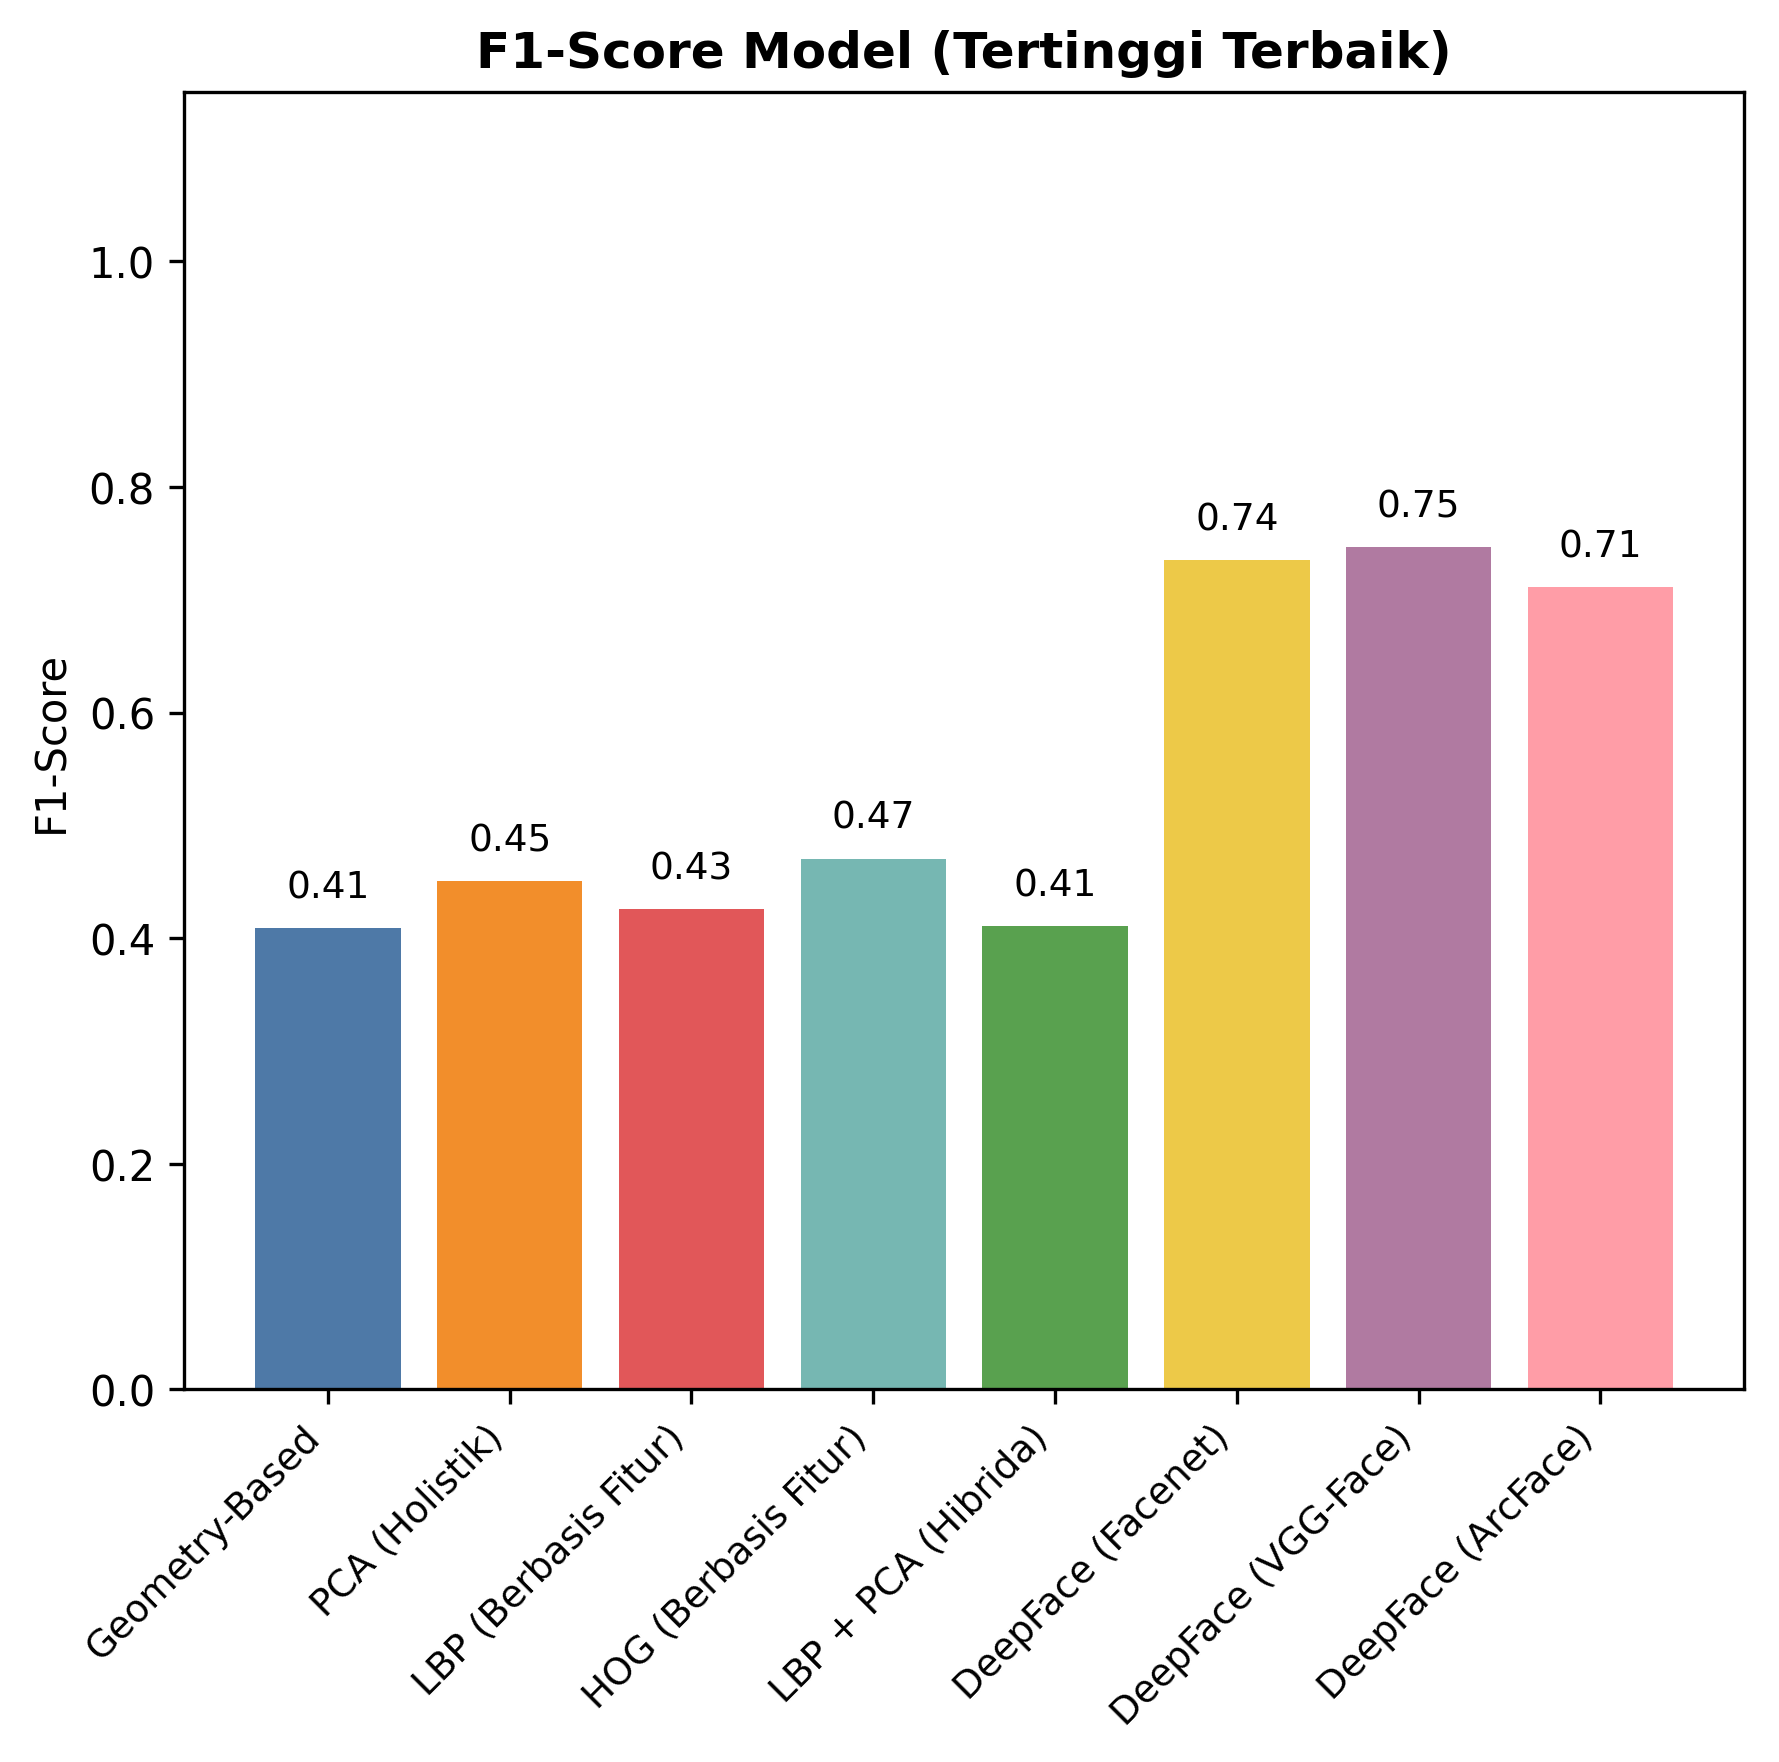
\includegraphics[width=0.85\textwidth]{images/b5-f1-score-mtcnn.png}
\end{figure}

\begin{figure}[h]
  \caption{Perbandingan F1-Score Seluruh Model dengan Detektor SCRFD}
  \label{fig:f1-score-scrfd}
  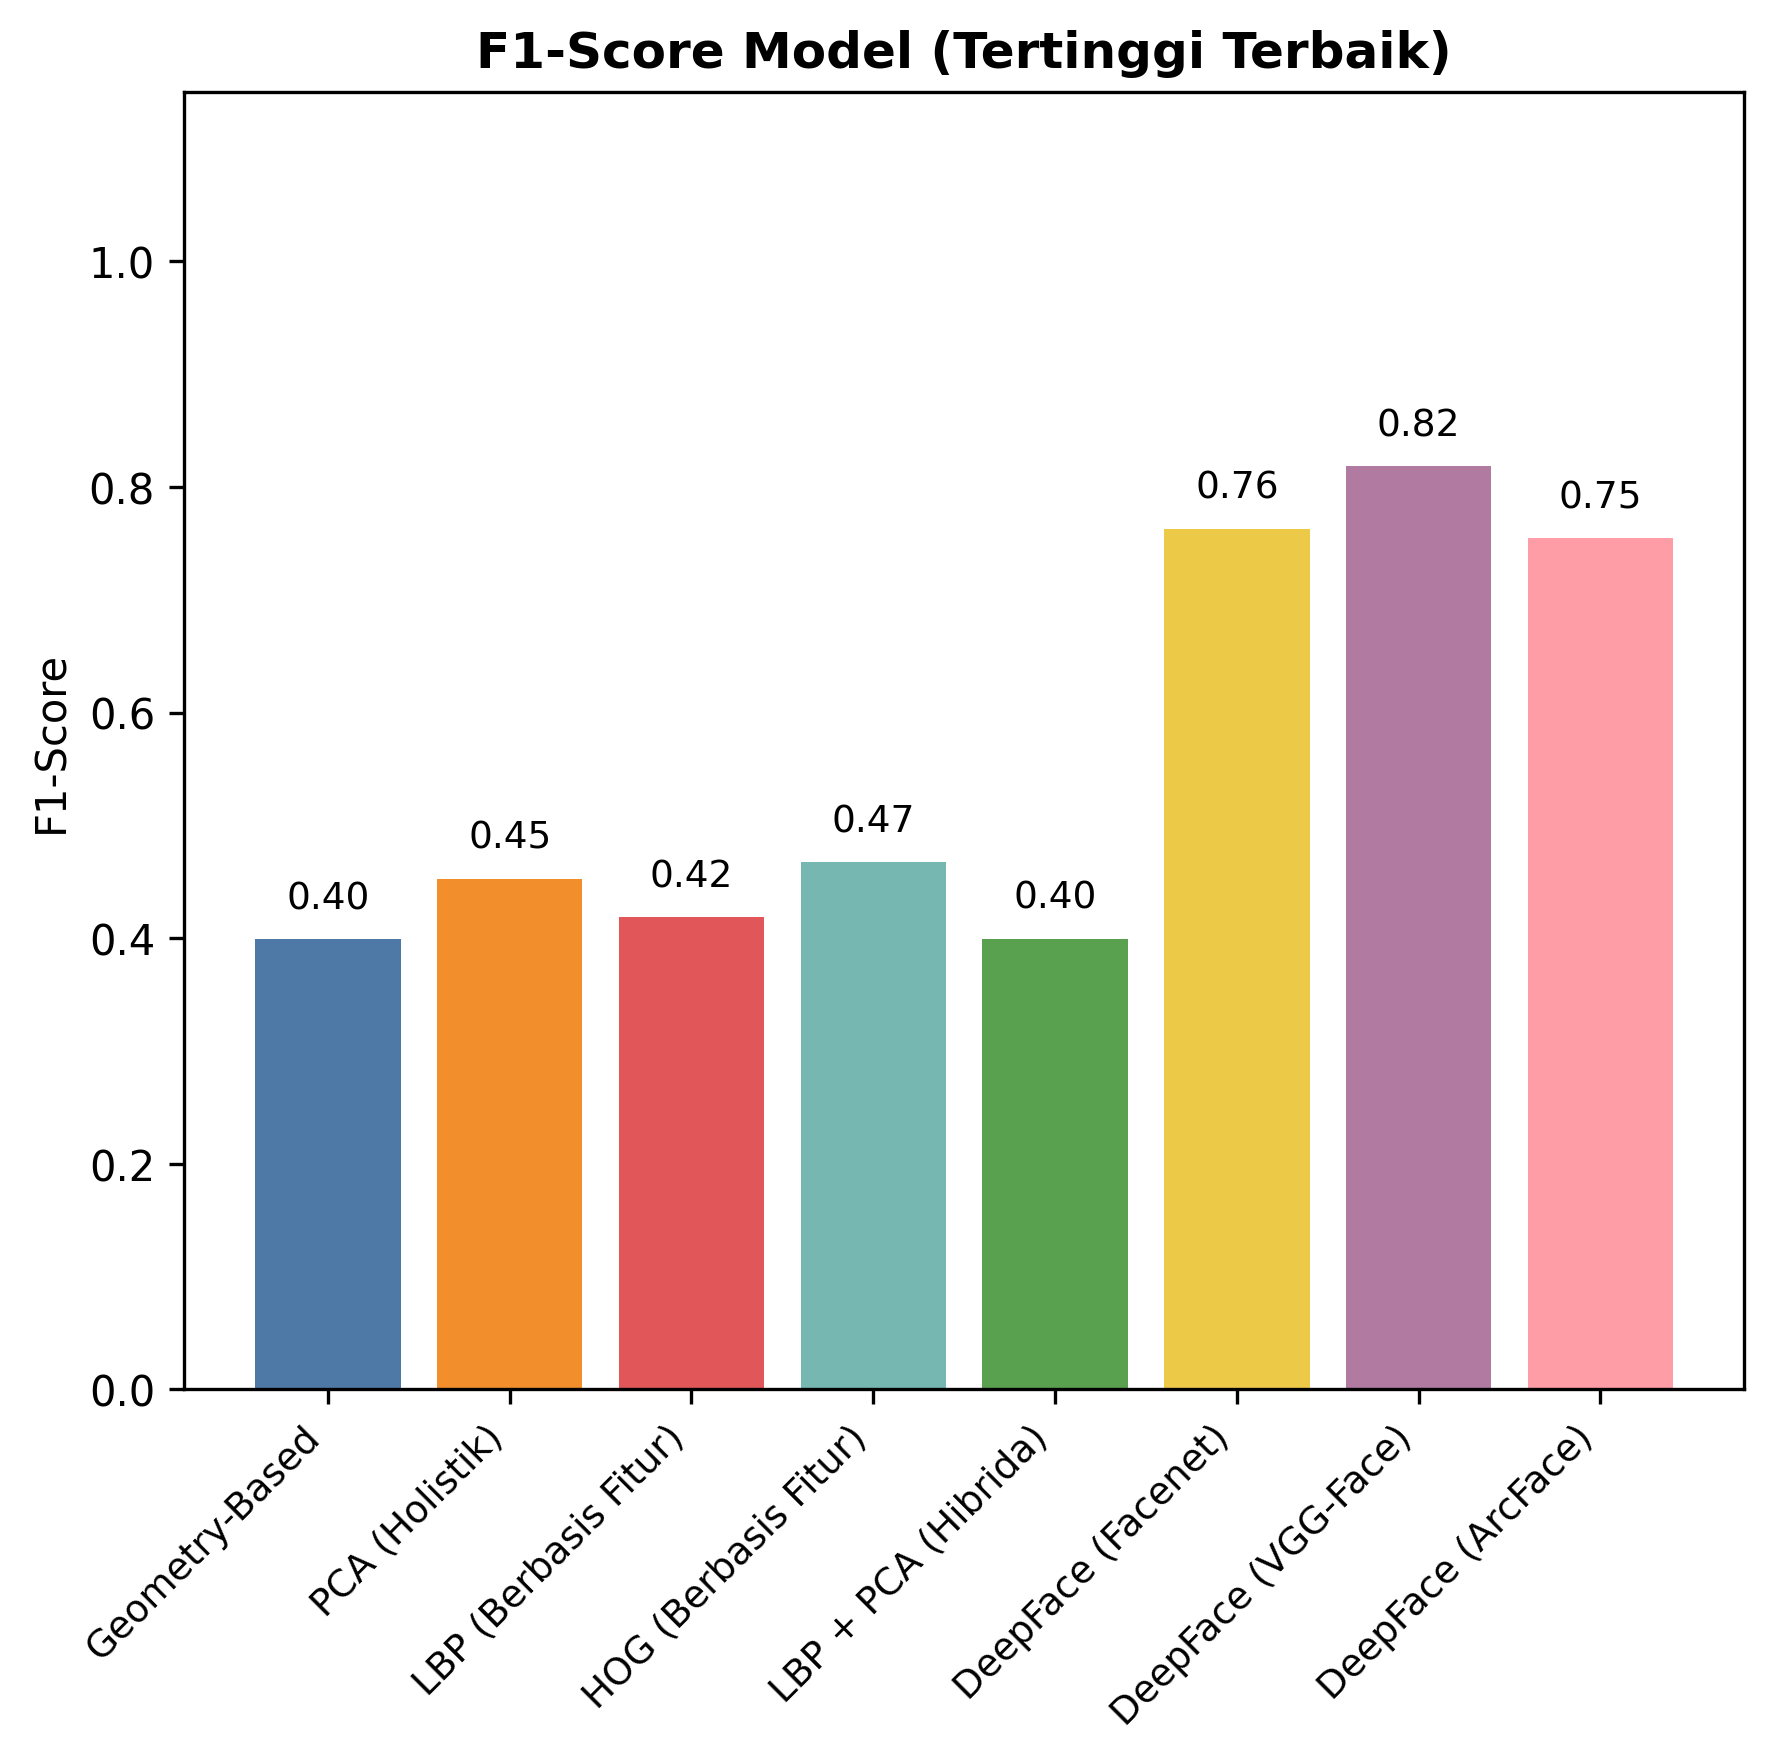
\includegraphics[width=0.85\textwidth]{images/b5-f1-score-scrfd.png}
\end{figure}

Gambar~\ref{fig:f1-score-mtcnn} dan Gambar~\ref{fig:f1-score-scrfd} menunjukkan bahwa metode berbasis \textit{deep learning} secara konsisten mendominasi peringkat F1-Score pada kedua konfigurasi detektor. Pada detektor MTCNN, tiga model teratas adalah \textit{VGG-Face} (0,747), \textit{FaceNet} (0,735), dan \textit{ArcFace} (0,711), jauh melampaui metode tradisional seperti HOG (0,471) dan PCA (0,451).

Penggunaan detektor SCRFD secara keseluruhan meningkatkan F1-Score seluruh model: \textit{VGG-Face} melonjak menjadi 0,819, \textit{FaceNet} menjadi 0,763, dan \textit{ArcFace} menjadi 0,755. Peningkatan ini mengindikasikan bahwa kualitas \textit{crop} wajah yang dihasilkan SCRFD lebih optimal sebagai masukan komponen \textit{embedding}, berkat presisi deteksi \textit{anchor-free} yang lebih akurat.

\subsection{Evaluasi Waktu Komputasi}

\begin{figure}[h]
  \caption{Perbandingan Waktu Komputasi Seluruh Model dengan Detektor MTCNN}
  \label{fig:waktu-mtcnn}
  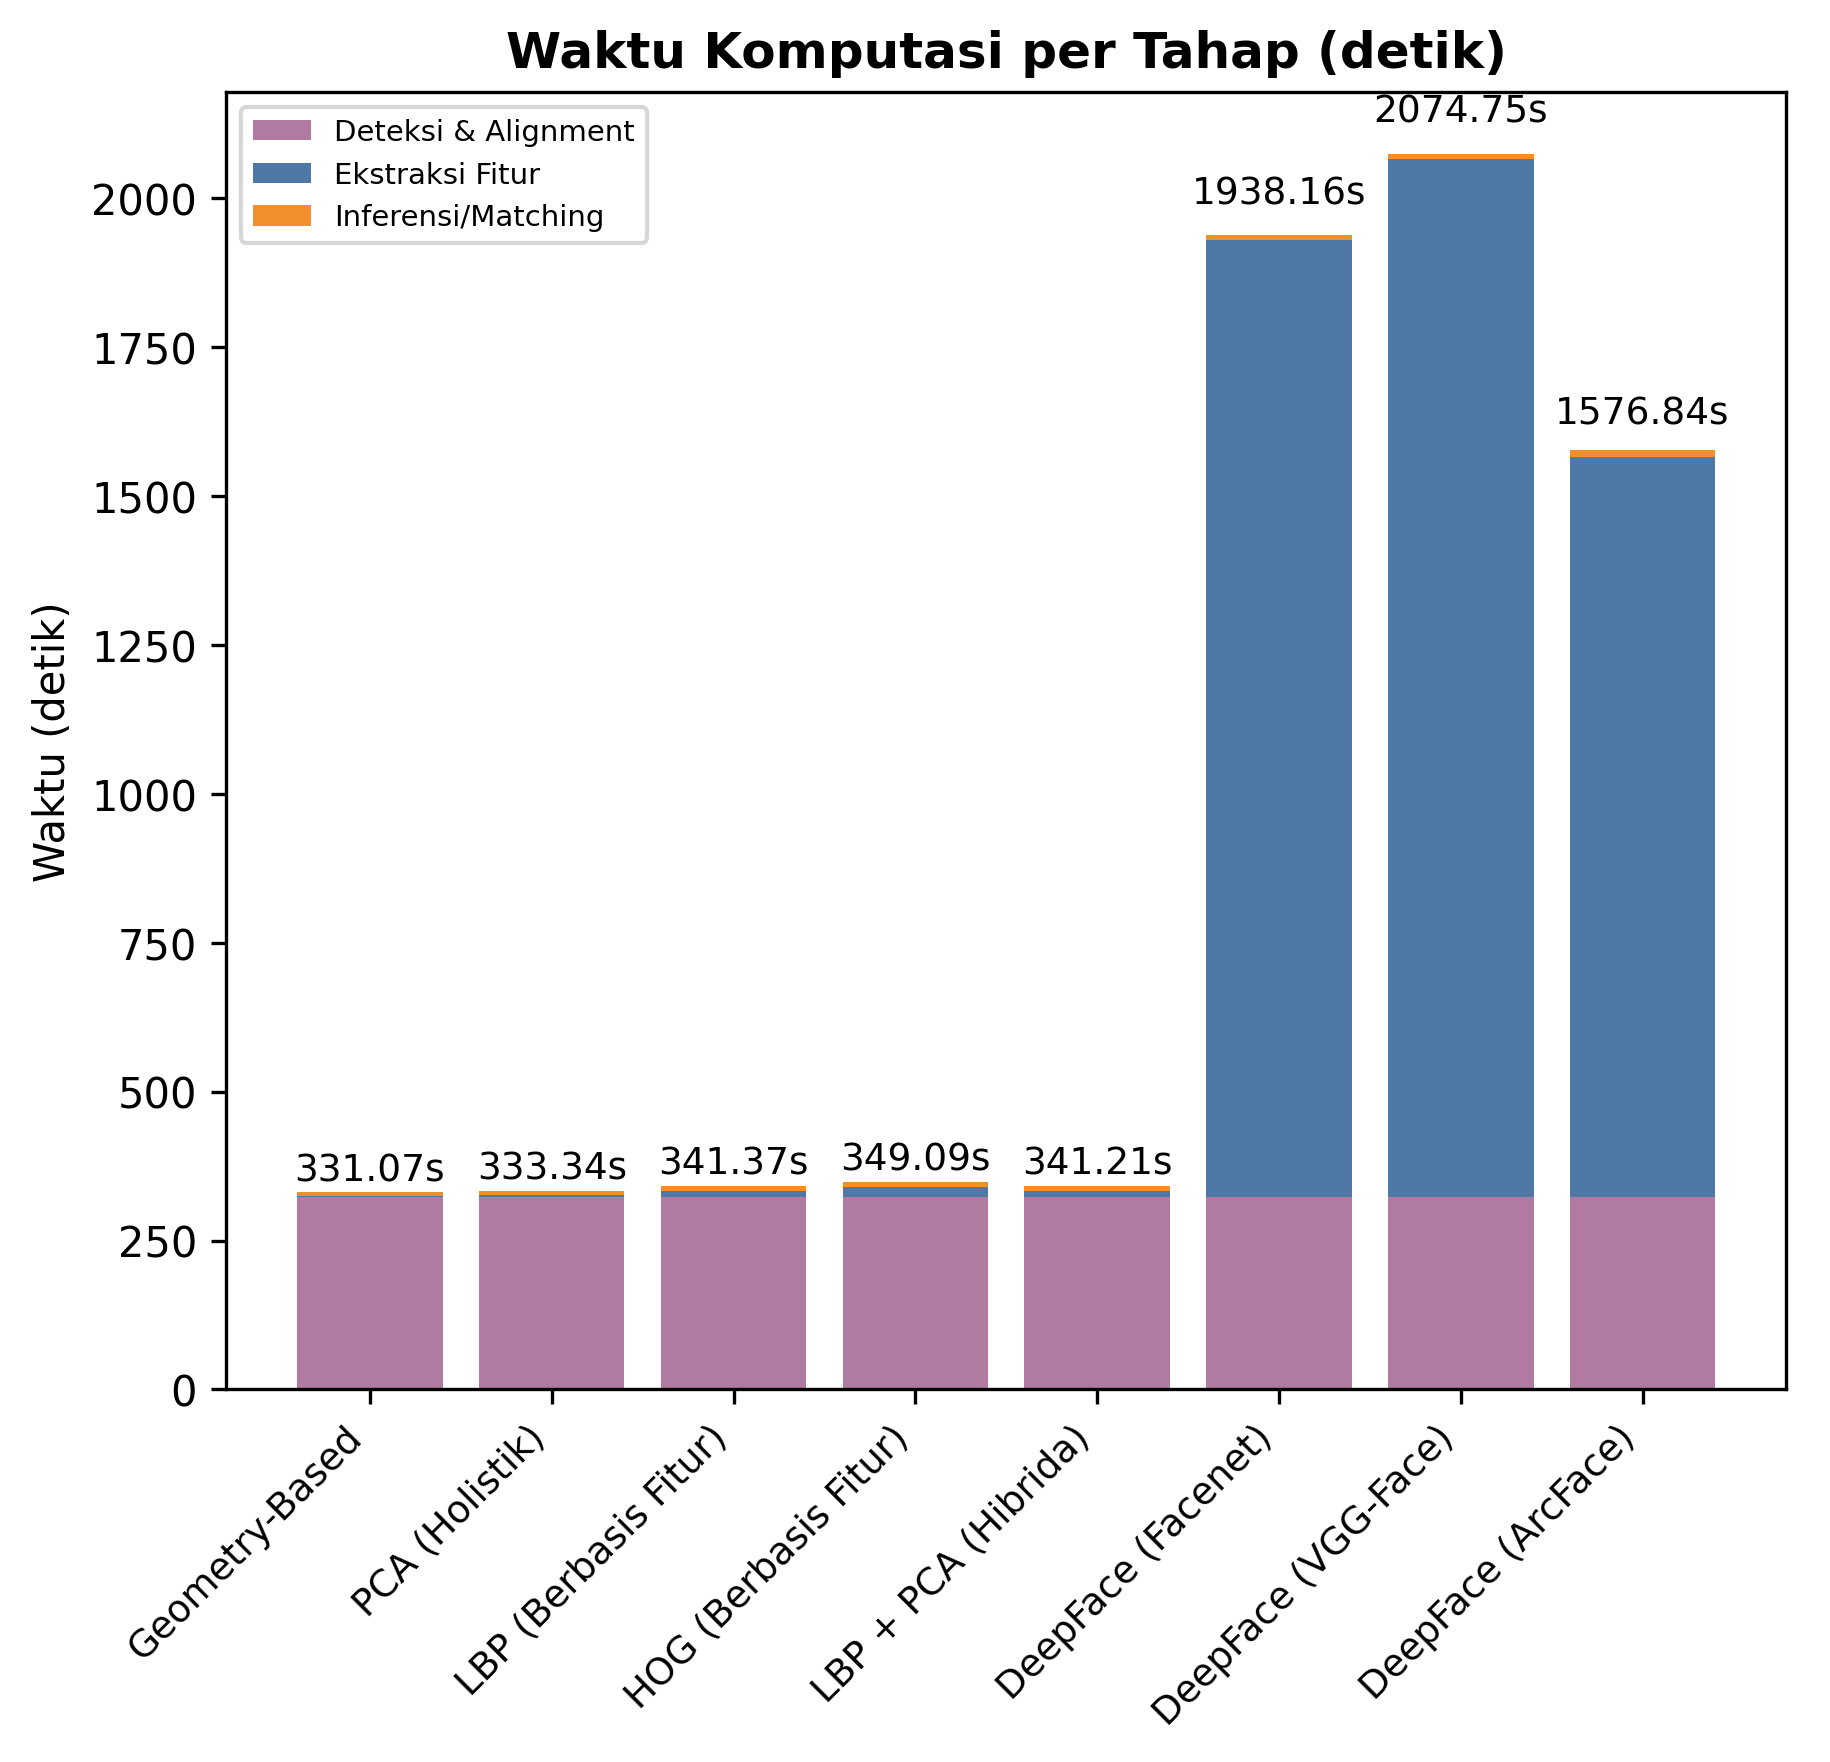
\includegraphics[width=0.85\textwidth]{images/b5-waktu-mtcnn.png}
\end{figure}

\begin{figure}[h]
  \caption{Perbandingan Waktu Komputasi Seluruh Model dengan Detektor SCRFD}
  \label{fig:waktu-scrfd}
  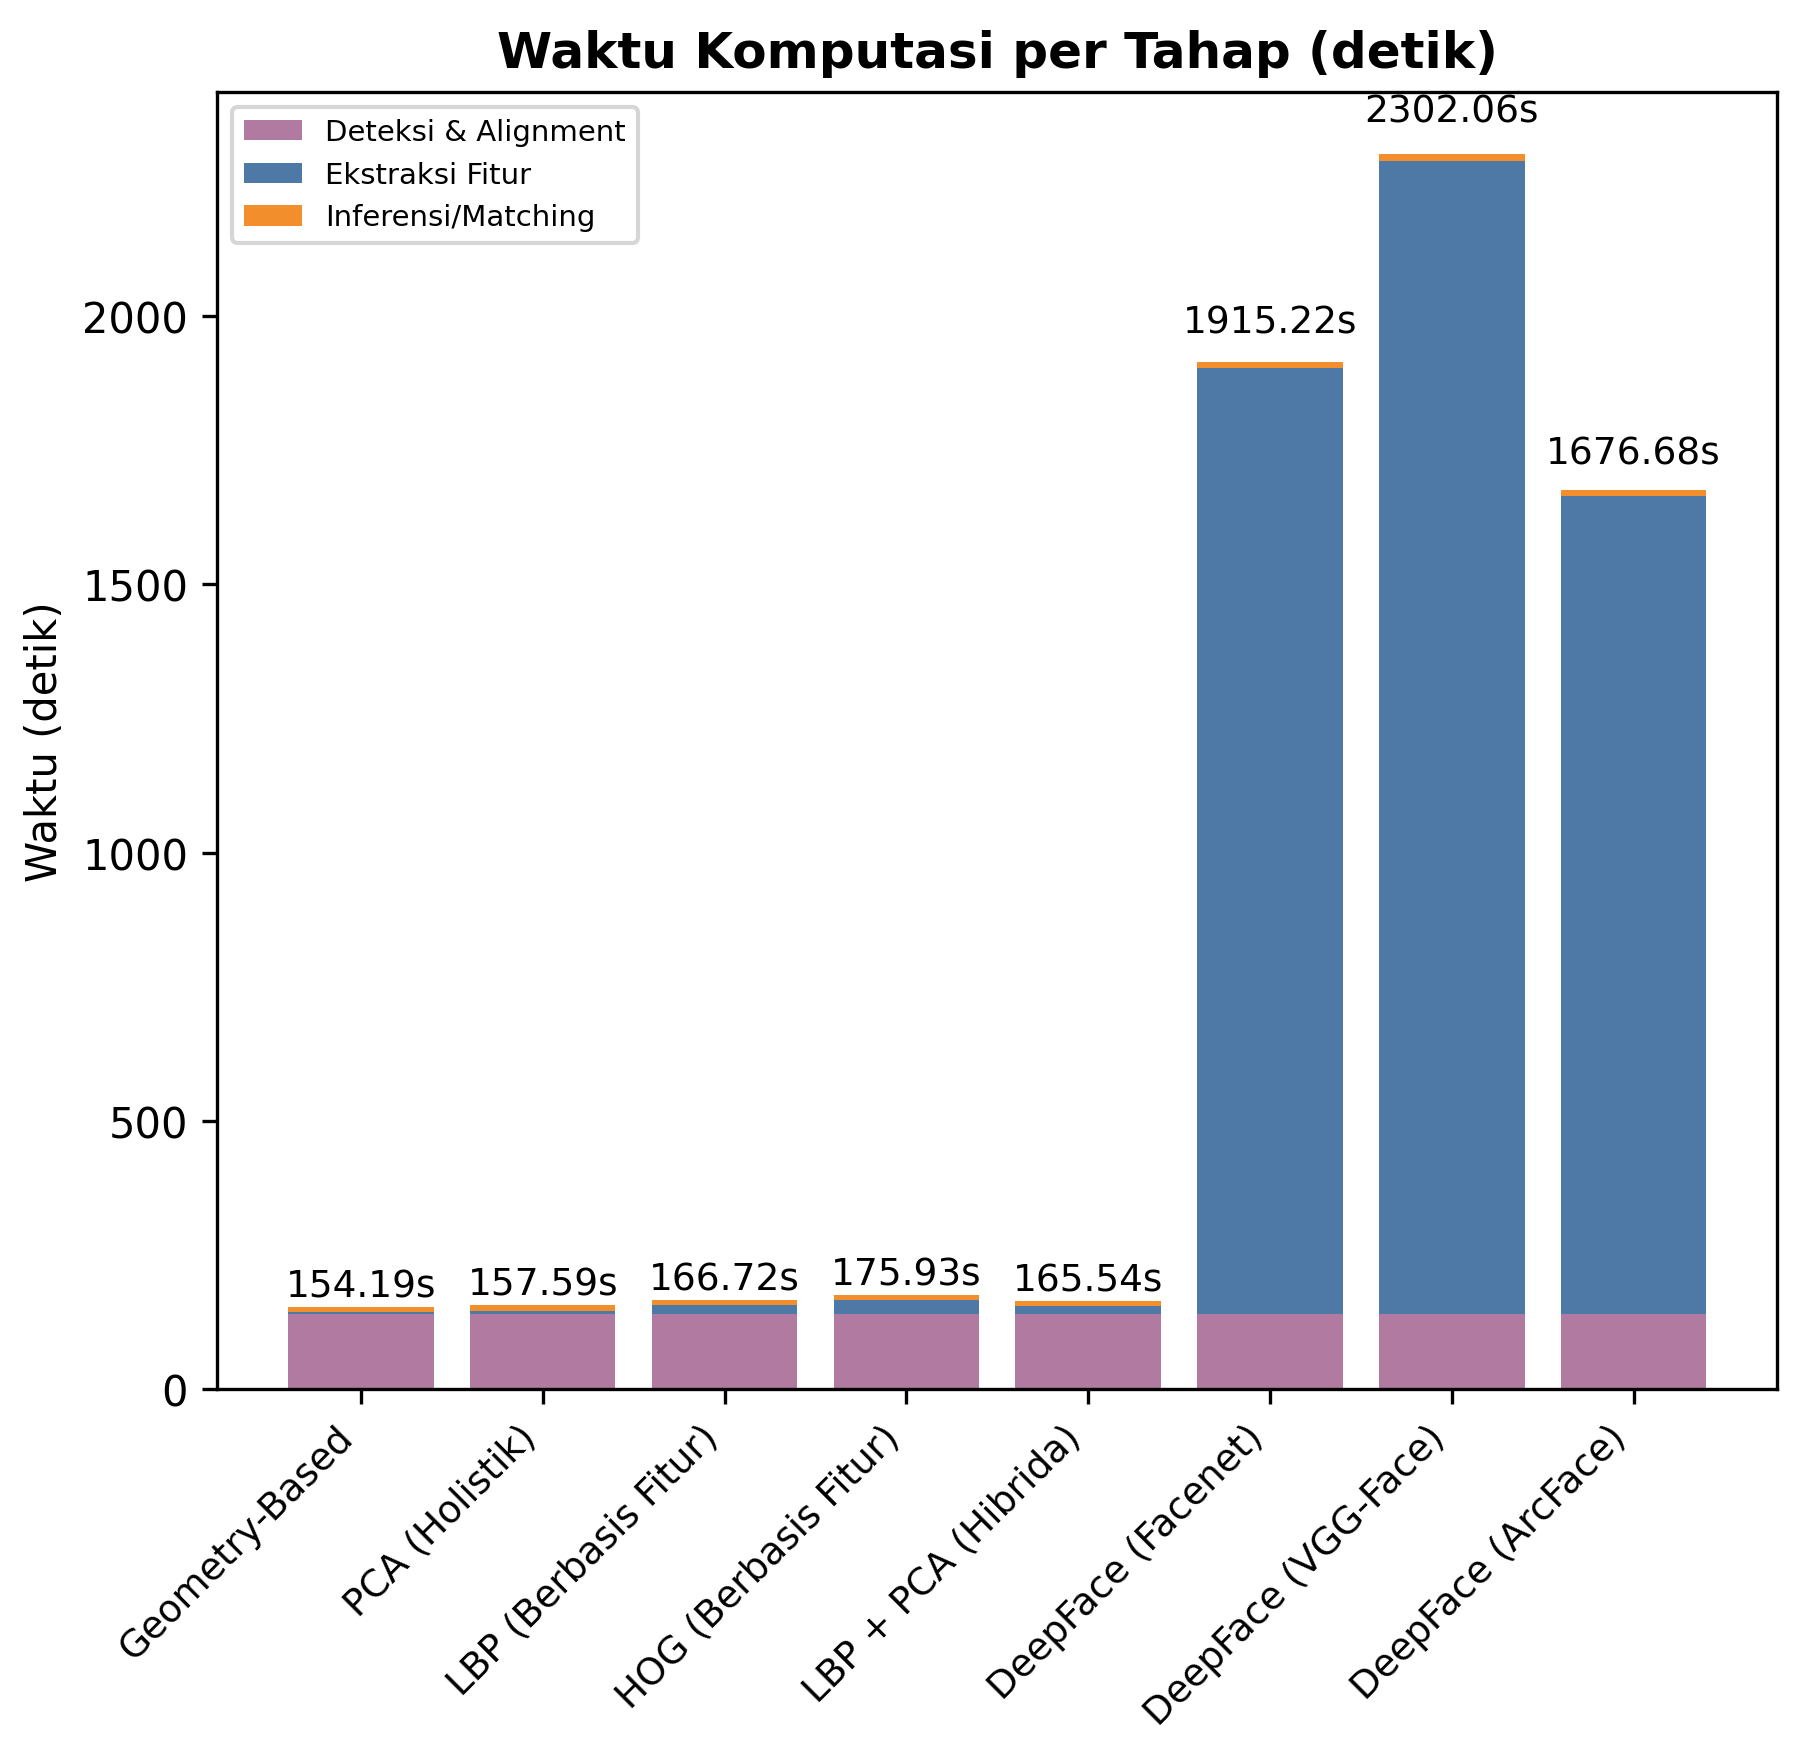
\includegraphics[width=0.85\textwidth]{images/b5-waktu-scrfd.png}
\end{figure}

Waktu deteksi MTCNN untuk 1.000 foto mencapai 322,40 detik, sedangkan SCRFD menyelesaikan tugas yang sama dalam 141,33 detik dengan percepatan sebesar $\pm 2{,}3\times$. Komponen ekstraksi fitur mendominasi total waktu pemrosesan pada metode \textit{deep learning}: \textit{ArcFace} membutuhkan sekitar 1.243 detik (MTCNN) dan 1.524 detik (SCRFD) untuk mengekstrak \textit{embedding} dari 1.000 foto via \textit{backend} DeepFace/TensorFlow.

Meskipun demikian, ekstraksi fitur merupakan \textit{one-time cost} yang hasilnya disimpan dalam \textit{cache} JSON, sehingga sesi pencarian berikutnya tidak memerlukan ekstraksi ulang. Metode tradisional (Geometri, LBP, HOG, PCA) memiliki waktu ekstraksi fitur yang jauh lebih singkat (di bawah 25 detik untuk 1.000 foto), namun nilai F1-Score yang rendah menjadikannya tidak memenuhi syarat minimal akurasi sistem.

\subsection{Evaluasi Penggunaan Memori}

\begin{figure}[h]
  \caption{Perbandingan Penggunaan Memori Seluruh Model dengan Detektor MTCNN}
  \label{fig:memory-mtcnn}
  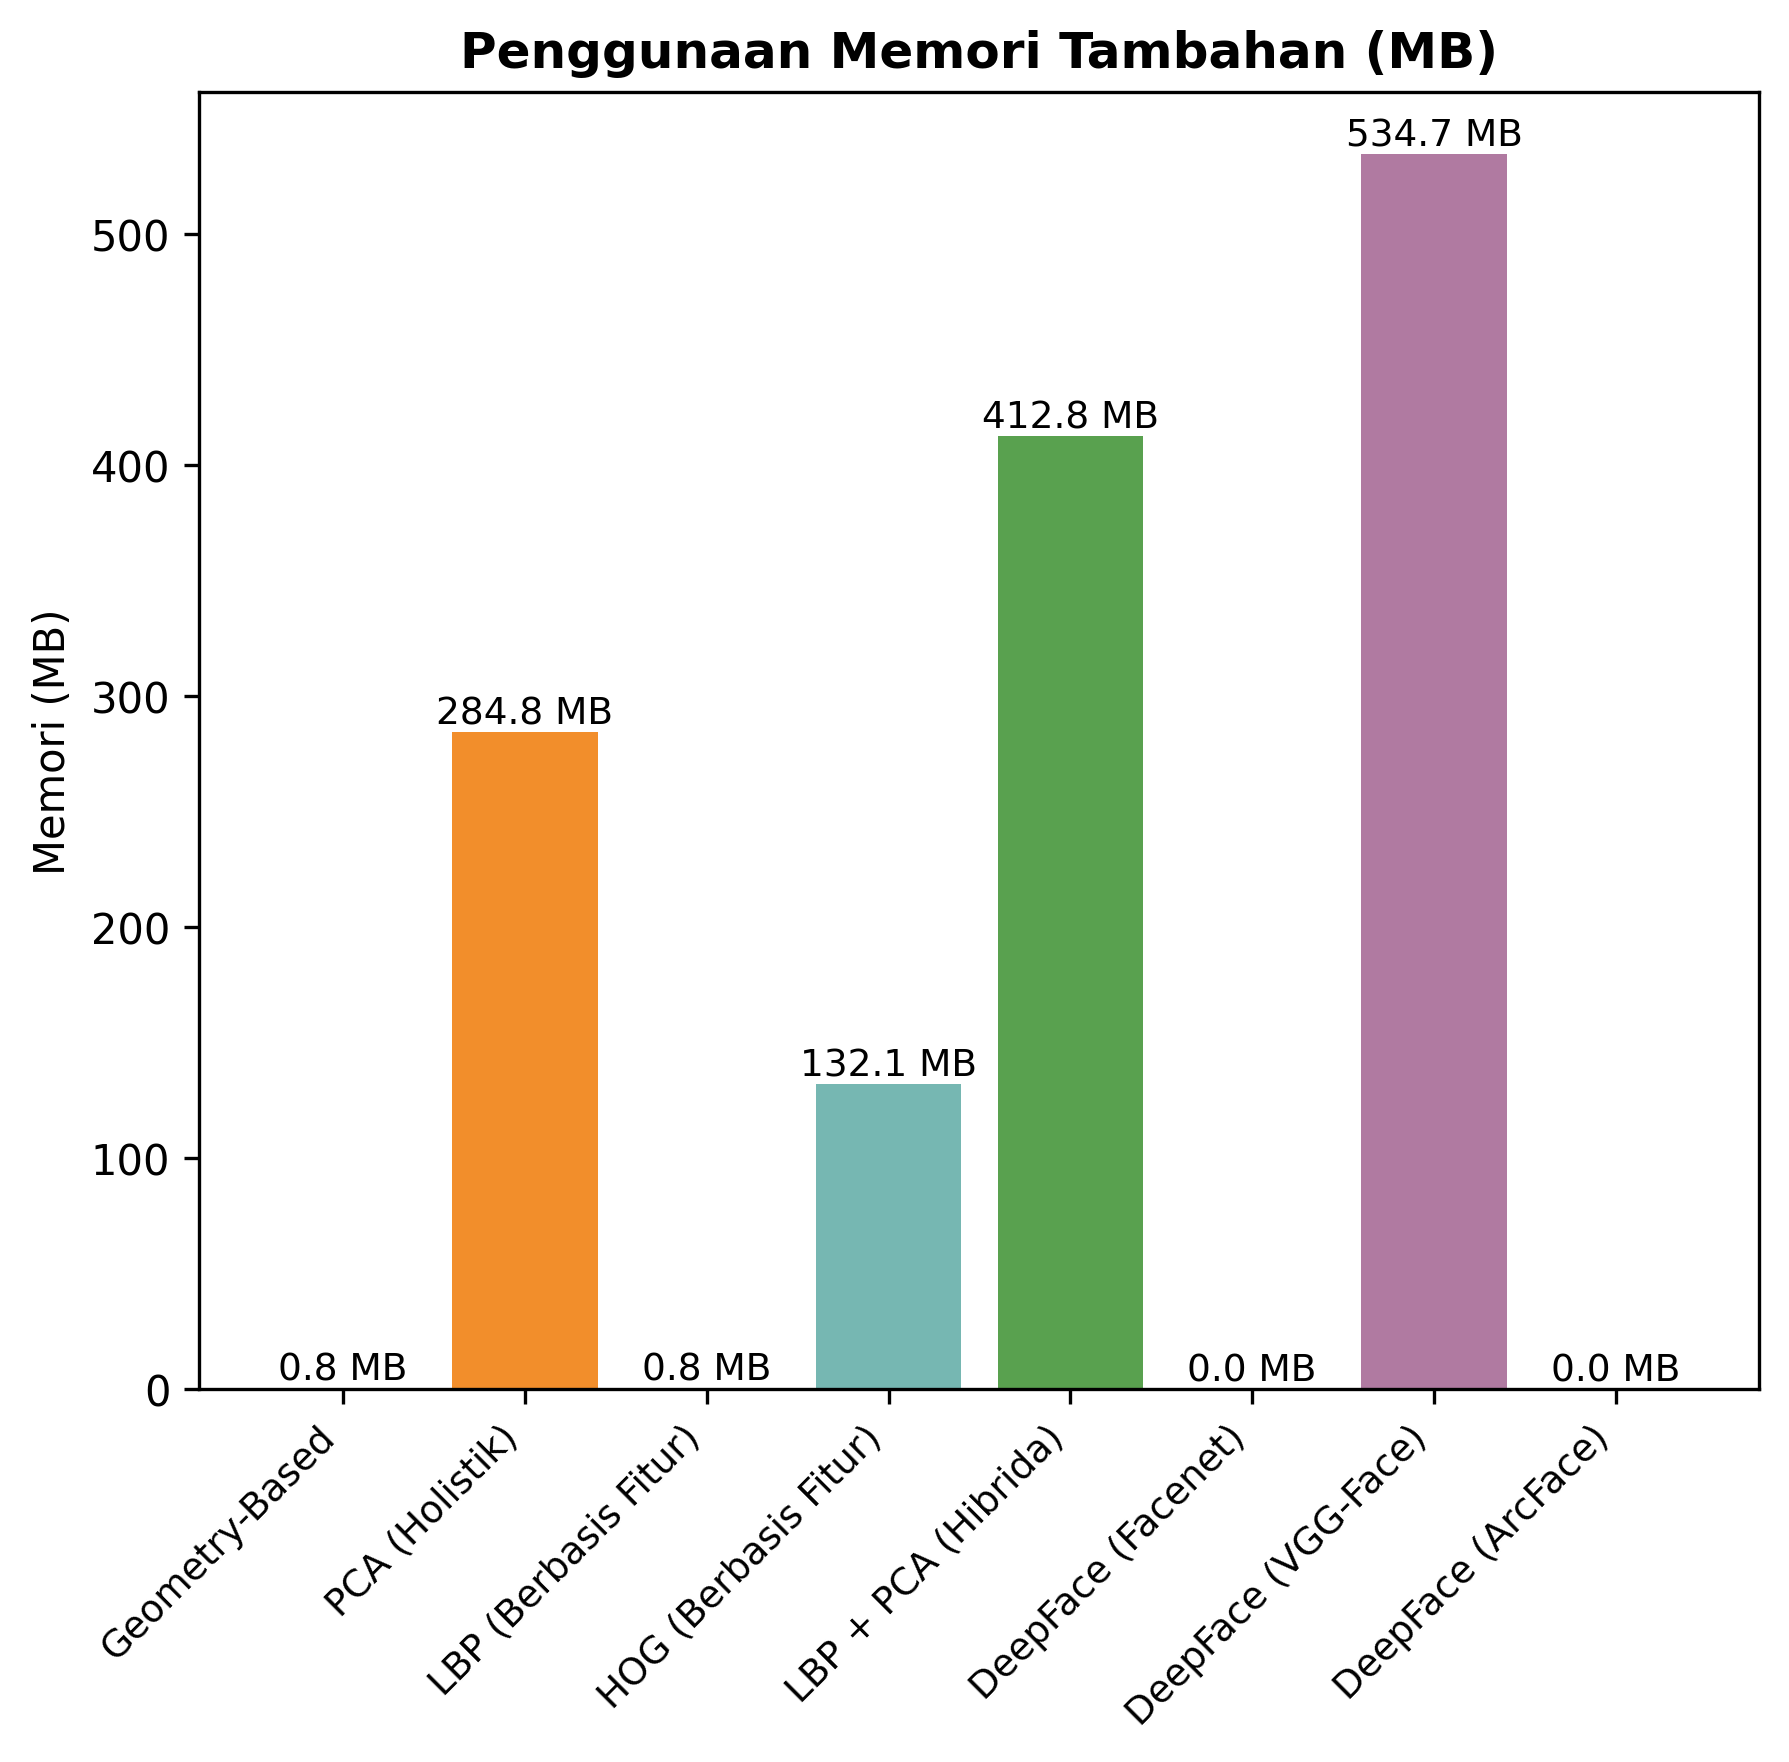
\includegraphics[width=0.85\textwidth]{images/b5-memory-mtcnn.png}
\end{figure}

\begin{figure}[h]
  \caption{Perbandingan Penggunaan Memori Seluruh Model dengan Detektor SCRFD}
  \label{fig:memory-scrfd}
  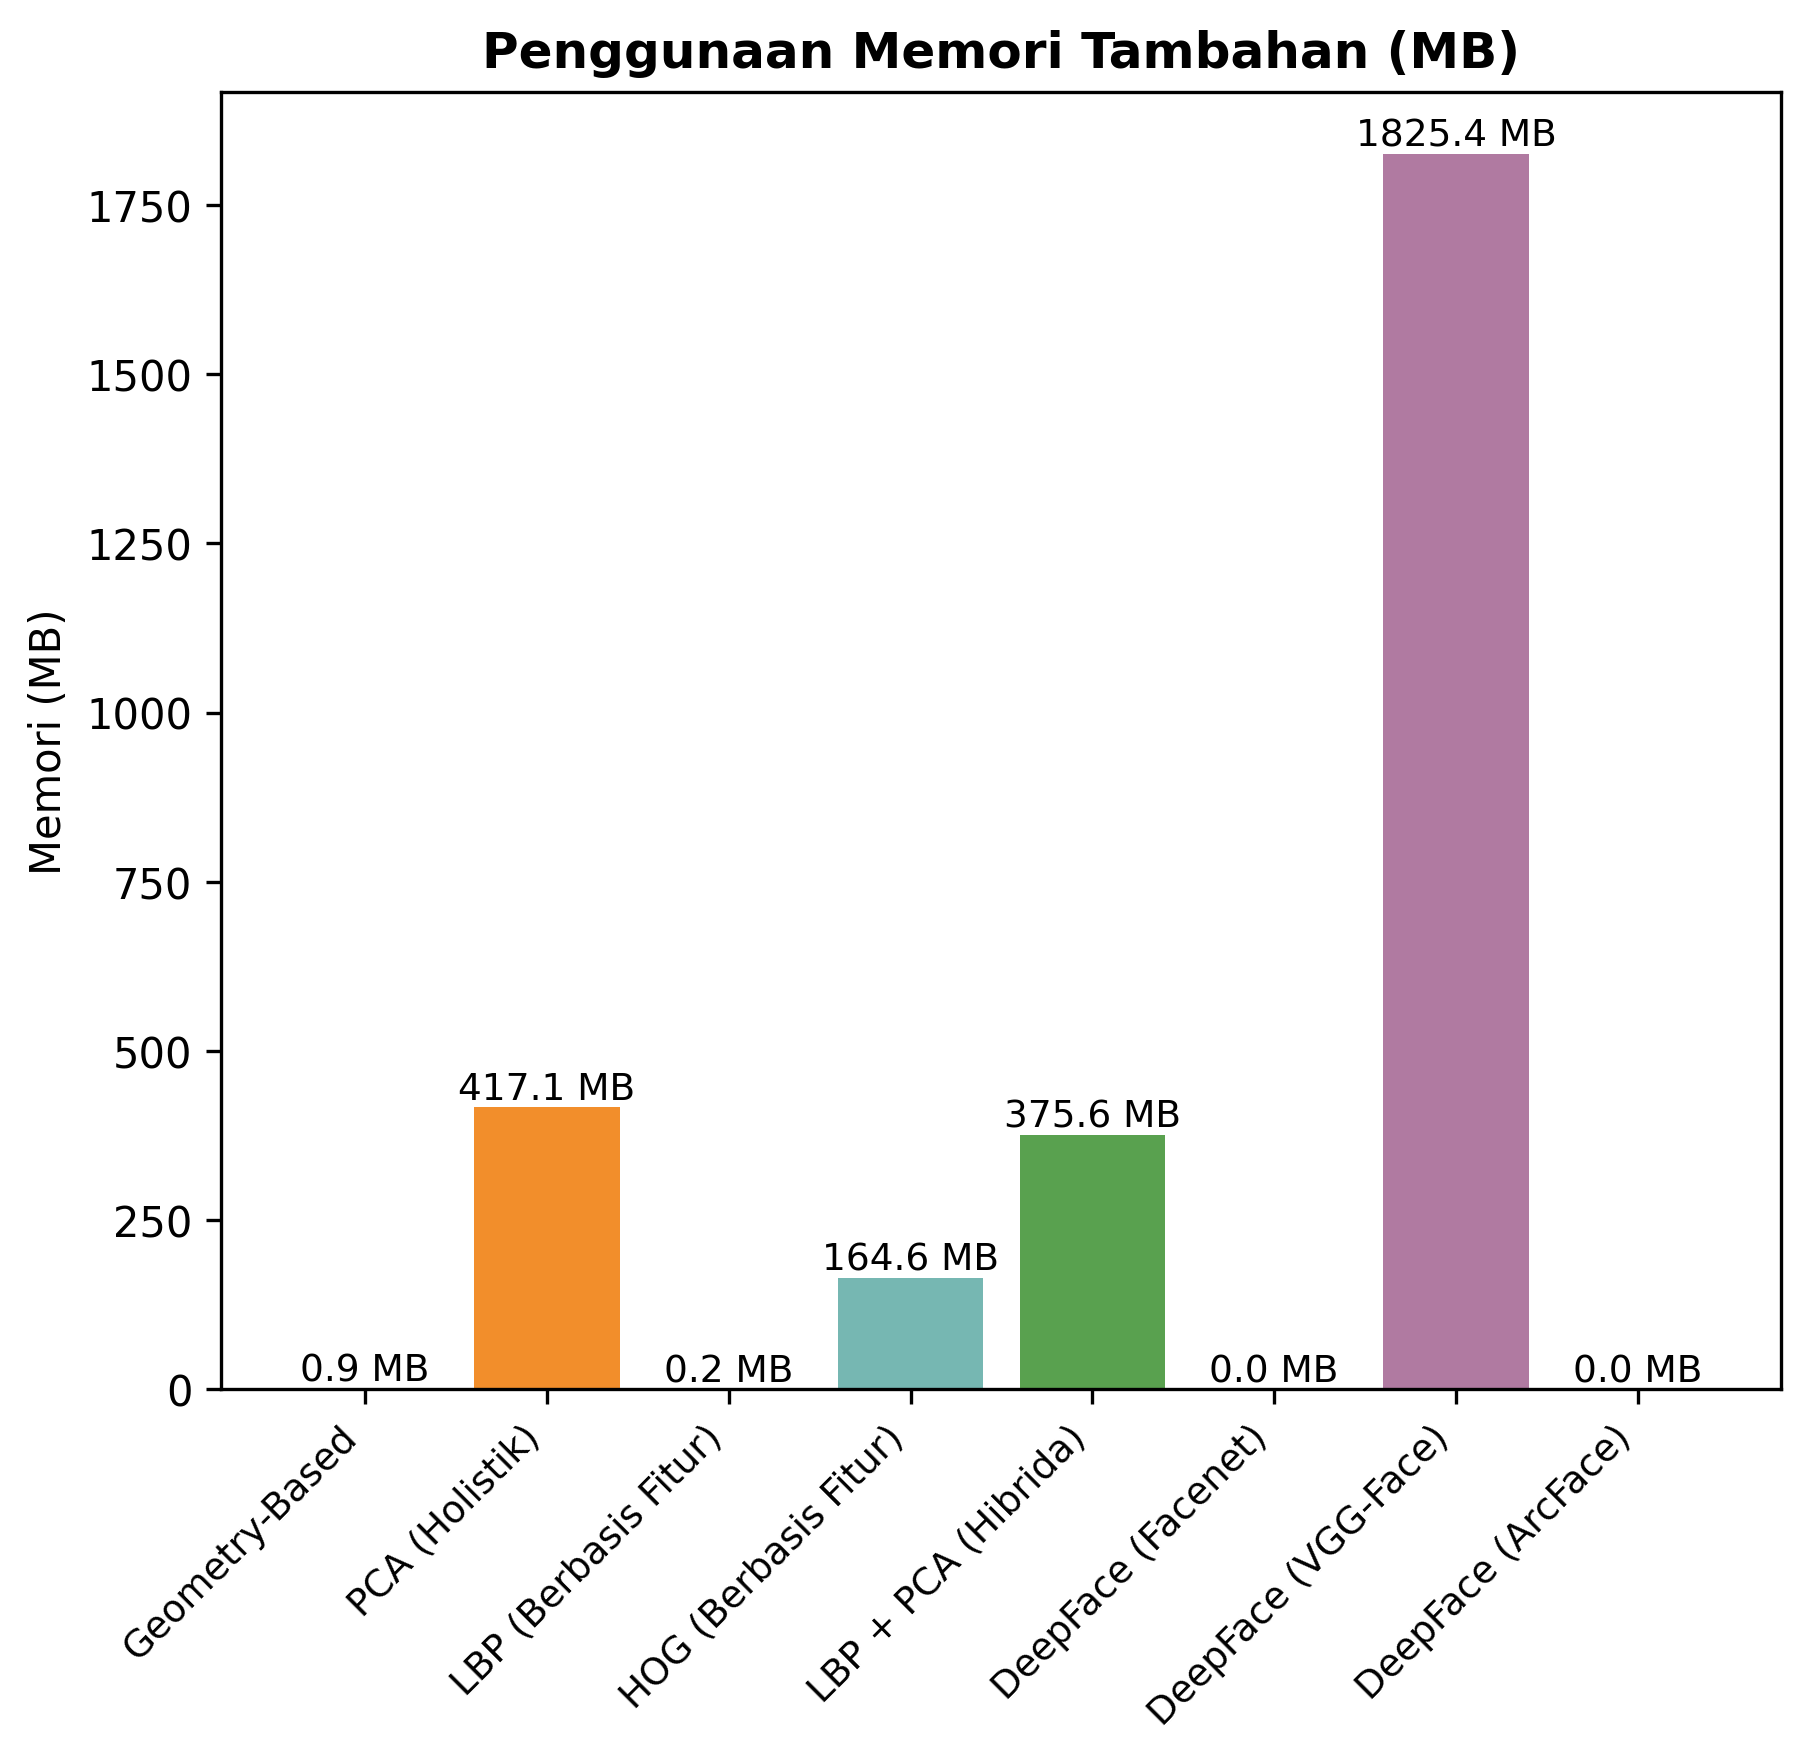
\includegraphics[width=0.85\textwidth]{images/b5-memory-scrfd.png}
\end{figure}

Kolom \textit{Memory Usage} pada Tabel~\ref{tab:hasil_perbandingan_lengkap} mencerminkan konsumsi memori inkremental komponen representasi wajah saat memproses 1.000 foto. \textit{ArcFace} dan \textit{FaceNet} menunjukkan konsumsi memori inkremental mendekati nol (0,000 MB), karena representasi \textit{embedding} 512 dimensi berformat \texttt{float32} hanya memerlukan $\approx 2$ KB per wajah.
Sebaliknya, \textit{VGG-Face} mengonsumsi memori inkremental yang sangat besar: 534,73 MB (MTCNN) dan 1.825,36 MB (SCRFD), akibat alokasi \textit{buffer intermediate activation} TensorFlow yang proporsional terhadap arsitektur model yang lebih dalam. Lonjakan drastis pada konfigurasi SCRFD menunjukkan bahwa resolusi \textit{crop} yang lebih tinggi dari SCRFD memperbesar alokasi tensor internal VGG-Face secara signifikan.

\subsection{Hasil Perbandingan Lengkap}

\begin{sidewaystable}[h]
    \centering
    \caption{Hasil Perbandingan Lengkap (8 Model) dengan Detektor MTCNN dan SCRFD}
    \label{tab:hasil_perbandingan_lengkap}

    % ---- Tabel 1: MTCNN ----
    \textbf{Tabel 1. Hasil Perbandingan dengan Detektor MTCNN}\\[0.5em]
    \begin{tabular}{|p{3cm}|p{1.5cm}|p{1.5cm}|p{1.5cm}|p{1.5cm}|p{1.5cm}|p{2.5cm}|p{2cm}|p{2cm}|p{2cm}|}
        \hline
        \textbf{Model} & \textbf{Accuracy} & \textbf{Precision} & \textbf{Recall} & \textbf{F1-Score} & \textbf{Best Threshold} & \textbf{Feature Extraction Time (s)} & \textbf{Inference Time (s)} & \textbf{Memory Usage (MB)} & \textbf{Detection Time (s)} \\ \hline

        Geometry-Based      & 0.345000 & 0.259557 & 0.960396 & 0.408667 & 0.05 & 1.794549    & 6.875577  & 0.796875   & 322.398885 \\ \hline
        PCA (Holistik)      & 0.547667 & 0.315760 & 0.787836 & 0.450830 & 0.95 & 3.439454    & 7.505657  & 284.753906 & 322.398885 \\ \hline
        LBP (Berbasis Fitur)& 0.441333 & 0.280868 & 0.878359 & 0.425634 & 0.25 & 11.494441   & 7.472873  & 0.781250   & 322.398885 \\ \hline
        HOG (Berbasis Fitur)& 0.574000 & 0.332748 & 0.803395 & 0.470588 & 0.30 & 18.239864   & 8.448654  & 132.109375 & 322.398885 \\ \hline
        LBP + PCA (Hibrida) & 0.459333 & 0.276284 & 0.799151 & 0.410610 & 0.95 & 11.062305   & 7.749343  & 412.812500 & 322.398885 \\ \hline
        DeepFace (Facenet)  & 0.874333 & 0.730447 & 0.739745 & 0.735067 & 0.40 & 1607.450316 & 8.306349  & 0.000000   & 322.398885 \\ \hline
        DeepFace (VGG-Face) & 0.894333 & 0.858456 & 0.660537 & 0.746603 & 0.60 & 1743.119371 & 9.228585  & 534.734375 & 322.398885 \\ \hline
        DeepFace (ArcFace)  & 0.861000 & 0.696477 & 0.727016 & 0.711419 & 0.65 & 1243.435217 & 11.005755 & 0.000000   & 322.398885 \\ \hline

    \end{tabular}

    \vspace{1.5em}

    % ---- Tabel 2: SCRFD ----
    \textbf{Tabel 2. Hasil Perbandingan dengan Detektor SCRFD}\\[0.5em]
    \begin{tabular}{|p{3cm}|p{1.5cm}|p{1.5cm}|p{1.5cm}|p{1.5cm}|p{1.5cm}|p{2.5cm}|p{2cm}|p{2cm}|p{2cm}|}
        \hline
        \textbf{Model} & \textbf{Accuracy} & \textbf{Precision} & \textbf{Recall} & \textbf{F1-Score} & \textbf{Best Threshold} & \textbf{Feature Extraction Time (s)} & \textbf{Inference Time (s)} & \textbf{Memory Usage (MB)} & \textbf{Detection Time (s)} \\ \hline

        Geometry-Based      & 0.290000 & 0.249207 & 1.000000 & 0.398984 & 0.05 & 2.854128    & 10.009302 & 0.945312    & 141.329536 \\ \hline
        PCA (Holistik)      & 0.514333 & 0.308282 & 0.852900 & 0.452873 & 0.95 & 5.522211    & 10.739054 & 417.066406  & 141.329536 \\ \hline
        LBP (Berbasis Fitur)& 0.372000 & 0.267850 & 0.960396 & 0.418877 & 0.30 & 15.818657   & 9.571036  & 0.203125    & 141.329536 \\ \hline
        HOG (Berbasis Fitur)& 0.587667 & 0.336015 & 0.768034 & 0.467499 & 0.30 & 24.706835   & 9.894295  & 164.617188  & 141.329536 \\ \hline
        LBP + PCA (Hibrida) & 0.408000 & 0.262550 & 0.835926 & 0.399594 & 0.95 & 14.041398   & 10.164680 & 375.601562  & 141.329536 \\ \hline
        DeepFace (Facenet)  & 0.889000 & 0.767908 & 0.758133 & 0.762989 & 0.40 & 1761.458499 & 12.435488 & 0.000000    & 141.329536 \\ \hline
        DeepFace (VGG-Face) & 0.922000 & 0.905660 & 0.746818 & 0.818605 & 0.60 & 2147.132272 & 13.597491 & 1825.359375 & 141.329536 \\ \hline
        DeepFace (ArcFace)  & 0.891000 & 0.803514 & 0.711457 & 0.754689 & 0.60 & 1524.226980 & 11.120317 & 0.000000    & 141.329536 \\ \hline

    \end{tabular}

\end{sidewaystable}

Tabel~\ref{tab:hasil_perbandingan_lengkap} merangkum seluruh metrik evaluasi dari delapan model pada kedua konfigurasi detektor. Secara umum, detektor SCRFD menghasilkan performa yang lebih baik hampir pada semua model dibandingkan MTCNN, baik dari sisi akurasi, F1-Score, maupun kecepatan deteksi, sehingga SCRFD menjadi kandidat detektor yang lebih unggul untuk sistem produksi.

\section{Algoritma yang Dipilih}

Berdasarkan hasil analisis komparatif di atas, \textbf{ArcFace} dipilih sebagai algoritma representasi wajah dan \textbf{SCRFD} dipilih sebagai detektor wajah pada sistem produksi. Pemilihan ini didasarkan pada argumen berikut:

\begin{enumerate}
    \item \textbf{Keseimbangan Optimal antara Akurasi dan Efisiensi Memori}

    Dengan detektor SCRFD, \textit{ArcFace} mencapai akurasi $89{,}1\%$ dan F1-Score $0{,}755$, sehingga memenuhi indikator keberhasilan nonfungsional minimal $85\%$ pada Tabel~\ref{tab:kebutuhan nonfungsional}. \textit{VGG-Face} memang menghasilkan akurasi lebih tinggi ($92{,}2\%$) dan F1-Score $0{,}819$, namun disertai konsumsi memori inkremental sebesar $1.825{,}36$ MB, lebih dari $400\times$ lebih besar dibandingkan \textit{ArcFace}. Untuk konteks aplikasi \textit{desktop offline} yang menargetkan perangkat dengan sumber daya terbatas, beban memori sebesar itu tidak dapat diterima.

    \item \textbf{Keunggulan Arsitektur \textit{Additive Angular Margin Loss}}

    Keunggulan utama \textit{ArcFace} terletak pada fungsi ruginya yang mendistribusikan \textit{face embedding} berdasarkan margin sudut (\textit{angular margin}) di ruang hiperbolik. Mekanisme ini menghasilkan representasi fitur yang lebih diskriminatif dibandingkan metode berbasis \textit{softmax} konvensional, sehingga lebih tangguh terhadap variasi pencahayaan, pose \textit{candid}, dan kondisi wajah tertutup sebagian pada foto dokumentasi riil.

    \item \textbf{Kompatibilitas ONNX Runtime}

    Model \textit{ArcFace} tersedia dalam format ONNX (\texttt{w600k\_r50.onnx}), memungkinkan inferensi langsung melalui ONNX Runtime tanpa ketergantungan pada TensorFlow. Migrasi ini menghasilkan peningkatan kecepatan inferensi \textit{embedding} sebesar $\pm 10$–$15\times$ (dari 0,15–0,25 detik menjadi 0,008–0,020 detik per wajah) dan mengurangi waktu inisialisasi model dari 5–15 detik menjadi kurang dari 1 detik.
\end{enumerate}

Argumen pemilihan SCRFD didasarkan pada kecepatan deteksi yang $\pm 2{,}3\times$ lebih cepat dibandingkan MTCNN (141,33 detik vs 322,40 detik untuk 1.000 foto), kualitas \textit{landmark} 5 titik yang setara, serta konsistensi \textit{backend}. SCRFD juga tersedia dalam format ONNX (\texttt{det\_2.5g.onnx}) sehingga sistem produksi cukup bergantung pada satu mesin inferensi tunggal.

Dengan demikian, sistem produksi mengintegrasikan kombinasi komponen berikut:

\begin{enumerate}
    \item \textbf{SCRFD} (\texttt{det\_2.5g.onnx}) sebagai komponen deteksi wajah
    \item \textbf{ArcFace ResNet-50} (\texttt{w600k\_r50.onnx}) sebagai komponen ekstraksi \textit{embedding} 512 dimensi
    \item \textbf{ONNX Runtime} (\texttt{CPUExecutionProvider}) sebagai mesin inferensi untuk kedua model di atas
\end{enumerate}

\section{Implementasi Sistem Produksi}

Sistem produksi diimplementasikan sebagai aplikasi desktop \textit{offline} sepenuhnya. Seluruh inferensi model, manajemen \textit{cache}, dan penyalinan hasil dilakukan secara lokal di perangkat pengguna.

\subsection{Arsitektur Komponen Perangkat Lunak}

Sistem diorganisasi ke dalam tiga lapisan komponen:

\begin{enumerate}
    \item \textbf{Lapisan GUI} (\texttt{src/gui/}): Antarmuka pengguna berbasis CustomTkinter dengan dua mode: mode produksi (\texttt{main.py}, \textit{threshold} tetap $\tau = 0{,}60$) dan mode demonstrasi (\texttt{main\_demo.py}, \textit{threshold} dapat diatur melalui \textit{slider} 0,10–1,00, dilengkapi pelaporan metrik evaluasi). Kelas \texttt{DemoApp} mewarisi (\textit{inherits}) dari \texttt{MainApp} dan hanya menimpa (\textit{overrides}) komponen yang berbeda.

    \item \textbf{Lapisan Inti} (\texttt{src/core/}): Tiga komponen \textit{stateless} yang dapat digunakan secara independen:
    \begin{enumerate}
        \item \texttt{FaceDetector}
        
        Deteksi wajah dengan SCRFD atau MTCNN, dilengkapi \textit{fallback} resolusi progresif (960px $\rightarrow$ 720px $\rightarrow$ 512px $\rightarrow$ 360px) untuk menangani gambar beresolusi sangat tinggi
        \item \texttt{ArcFaceONNXRunner}
        
        Ekstraksi \textit{embedding} 512 dimensi via ONNX Runtime, mendukung \textit{batch inference}
        \item \texttt{FaceMatcher}
        
        Pencarian jarak kosinus tervektor menggunakan operasi perkalian matriks NumPy (\texttt{np.dot})
    \end{enumerate}

    \item \textbf{Lapisan Data} (\texttt{src/cache\_io/}, \texttt{src/utils/}): \texttt{CacheHandler} mengelola \textit{cache} JSON per-wajah di direktori \texttt{.face\_cache/}; \texttt{FileManager} mengelola pemindaian folder rekursif (mengecualikan \texttt{.face\_cache/} dan \texttt{Hasil\_Pencarian\_Selfie/}) dan penyalinan hasil.
\end{enumerate}

\subsection{Pemrosesan Latar Belakang dan \textit{Thread Safety}}

Operasi pengindeksan dan pencarian dijalankan di \textit{daemon thread} terpisah (\texttt{PipelineWorker} dan \texttt{SearchWorker}) agar antarmuka GUI tetap responsif selama pemrosesan berlangsung. Semua pembaruan \textit{widget} dari \textit{thread} latar belakang dilakukan melalui \texttt{root.after(0, callback)}, yang menjadwalkan \textit{callback} pada iterasi berikutnya dari \textit{event loop} Tkinter di \textit{thread} utama.

\subsection{Pengindeksan Inkremental dan Pemrosesan \textit{Chunk}}

Sistem mendukung pengindeksan inkremental: foto yang telah memiliki entri \textit{cache} dilewati secara otomatis pada sesi pengindeksan berikutnya. Kunci \textit{cache} berupa MD5 dari pasangan (\textit{nama\_file\_relatif}, \textit{bounding box}), sehingga bersifat \textit{location-agnostic} karena pemindahan folder tidak membatalkan \textit{cache}.

Foto baru diproses dalam kelompok (\textit{chunk}) berukuran $B = 16$ foto. Untuk setiap \textit{chunk}:

\begin{enumerate}
    \item Deteksi wajah dijalankan secara sekuensial untuk 16 foto
    \item Seluruh \textit{crop} wajah dari 16 foto dikumpulkan menjadi satu \textit{batch tensor} berukuran $(N_{\text{wajah}}, 3, 112, 112)$
    \item Satu pemanggilan \texttt{session.run()} mengekstrak \textit{embedding} untuk seluruh \textit{batch}
    \item Setiap \textit{embedding} disimpan ke \textit{cache} JSON segera setelah diekstrak
\end{enumerate}

Mekanisme ini mereduksi frekuensi pemanggilan \texttt{session.run()} dari $\mathcal{O}(N)$ menjadi $\mathcal{O}\left(\lceil \frac{N}{B} \rceil\right)$, yang secara signifikan mengurangi \textit{overhead} eksekusi ONNX Runtime.